\documentclass{beamer}

\usepackage{graphicx}
\usepackage[latin1]{inputenc}
\usepackage[T1]{fontenc}
\usepackage[english]{babel}
\usepackage{listings}
\usepackage{xcolor}
\usepackage{eso-pic}
\usepackage{mathrsfs}
\usepackage{url}
\usepackage{amssymb}
\usepackage{amsmath}
\usepackage{multirow}
\usepackage{hyperref}
\usepackage{booktabs}
% \usepackage{bbm}
\usepackage{cooltooltips}
\usepackage{colordef}
\usepackage{beamerdefs}
\usepackage{lvblisting}

\pgfdeclareimage[height=2cm]{logobig}{hulogo}
% Supply the correct logo for your class and change the file name to "logo". The logo will appear in the lower
% right corner:
\pgfdeclareimage[height=0.7cm]{logosmall}{sim_logo}

% Title page outline:
% use this number to modify the scaling of the headline on title page
\renewcommand{\titlescale}{1.0}
% the title page has two columns, the following two values determine the percentage each one should get
\renewcommand{\titlescale}{1.0}
\renewcommand{\leftcol}{0.6}

% Define the title.Don't forget to insert an abbreviation instead 
% of "title for footer". It will appear in the lower left corner:
\title[QML estimation of an ARCH(1) model:]{Monte Carlo simulation of a QML estimation of an ARCH(1) model}
% Define the authors:
\authora{Paulina Kurowska} % a-c
\authorb{Bingling Wang}
\authorc{}

% Define any internet addresses, if you want to display them on the title page:
\def\linka{https://github.com/QuantLet/SFE\_class\_2017}
\def\linkb{}
\def\linkc{}
% Define the institute:
\institute{Ladislaus von Bortkiewicz Chair of Statistics \\
	Humboldt--Universit�t zu Berlin \\}

% Comment the following command, if you don't want, that the pdf file starts in full screen mode:
\hypersetup{pdfpagemode=FullScreen}

%Start of the document
\begin{document}
	
	% create the title slide, layout controlled in beamerdefs.sty and the foregoing specifications
\frame[plain]{
	\titlepage
	}
	
	
	% The titles of the different sections of you talk, can be included via the \section command. The title will be displayed in the upper left corner. To indicate a new section, repeat the \section command with, of course, another section title
	%%%%%%%%%%%%%%%%%%%%%%%%%%%%%%%%%%%%%%%%%%%%%%%%%%%%%%%%%%%%%%%%%%%%%%%%%%%%%%%%%%%%%%%%%%%%%%%%%%%%%%%%%%%%%%%%%%%%%%%%
	\section{Introduction}
	%%%%%%%%%%%%%%%%%%%%%%%%%%%%%%%%%%%%%%%%%%%%%%%%%%%%%%%%%%%%%%%%%%%%%%%%%%%%%%%%%%%%%%%%%%%%%%%%%%%%%%%%%%%%%%%%%%%%%%%%
	
	% (A numbering of the slides can be useful for corrections, especially if you are
	% dealing with large tex-files)
	%%%%%%%%%%%%%%%%%%%%%%%%%%%%%%%%%%%%%%%%%%%%%%%%%%%%%%%%%%%%%%%%%%%%%%%%%%%%%%%%%%%%%%%%%%%%%%%%%%%%%%%%%%%%%%%%%%%%%%%%
	
	
	%%%%%%%%%%%%%%%%%%%%%%%%%%%%%%%%%%%%%%%%%%%%%%%%%%%%%%%%%%%%%%%%%%%%%%%%%%%%%%%%%%%%%%%%%%%%%%%%%%%%%%%%%%%%%%%%%%%%%%%%
	% No number on outline slide
	\section{outline}
	\useheadtemplate{%
		\raisebox{-0.75cm}{\parbox{\textwidth}{%
				\footnotesize{\color{isegray}%
					\insertsection\ \leavevmode\leaders\hrule height3.2pt depth-2.8pt\hfill\kern0pt\ }}}
	}
	
	\frame[containsverbatim]{
		\frametitle{Outline}
		
		\begin{enumerate}
			\item ARCH(1) model
			\item Maximum Likelihood estimation
			\item Quasi Maximum Likelihood estimation
			\item Monte Carlo Set up
			\item Monte Carlo Simulation
			\item Simulation Results
			\item Further information
		\end{enumerate}
	}
	
	%%%%%%%%%%%%%%%%%%%%%%%%%%%%%%%%%%%%%%%%%%%%%%%%%%%%%%%%%%%%%%%%%%%%%%%%%%%%%%%%%%%%%%%%%%%%%%%%%%%%%%%%%%%%%%%%%%%%%
	\section{ARCH(1) Model}
	
	%%%%%%%%%%%%%%%%%%%%%%%%%%%%%%%%%%%%%%%%%%%%%%%%%%%%%%%%%%%%%%%%%%%%%%%%%%%%%%%%%%%%%%%%%%%%%%%%%%%%%%%%%%%%%%%%%%%%%%%%
	\subsection{General ideas}
	%%%%%%%%%%%%%%%%%%%%%%%%%%%%%%%%%%%%%%%%%%%%%%%%%%%%%%%%%%%%%%%%%%%%%%%%%%%%%%%%%%%%%%%%%%%%%%%%%%%%%%%%%%%%%%%%%%%%%%%%
\frame[containsverbatim]{
	\frametitle{Simulated ARCH(1) process}
	Simulated ARCH(1) process with 1000 observations, \(\alpha<1\)
	\begin{center}
		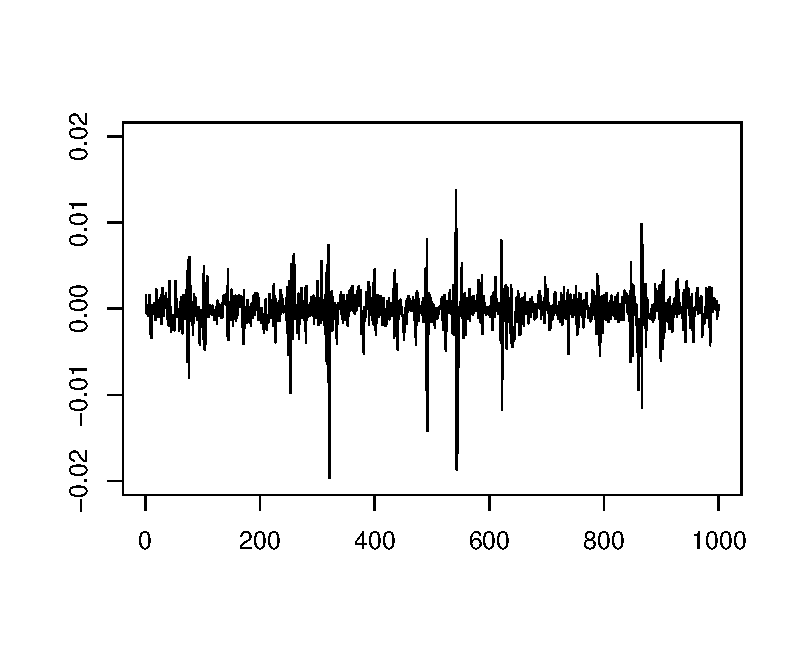
\includegraphics[scale=0.45]{ARCH(1)1.pdf}
	\end{center}
\hfill \includegraphics[scale=0.05]{qletlogo} \href{https://github.com/QuantLet/SFE\_class\_2017/tree/master/SFMqmle}{ SFMqmle}
	}	

	%%%%%%%%%%%%%%%%%%%%%%%%%%%%%%%%%%%%%%%%%%%%%%%%%%%%%%%%%%%%%%%%%%%%%%%%%%%%%%%%%%%%%%%%%%%%%%%%%%%%%%%%%%%%%%%%%%%%%%%%
\frame[containsverbatim]{
	\frametitle{Estimation of ARCH(1) Models}
	
	%\begin{itemize}
	 ARCH(1) process  \(\varepsilon_{t}\) has an AR(1) representation:
		\begin{eqnarray*}
			\varepsilon_{t}^{2}=\omega+\alpha\varepsilon_{t-1}^{2}+\eta_{t}, \eta_{t}=\sigma_{t}^{2}(Z_{t}^{2}-1)
		\end{eqnarray*}
	\begin{center}
		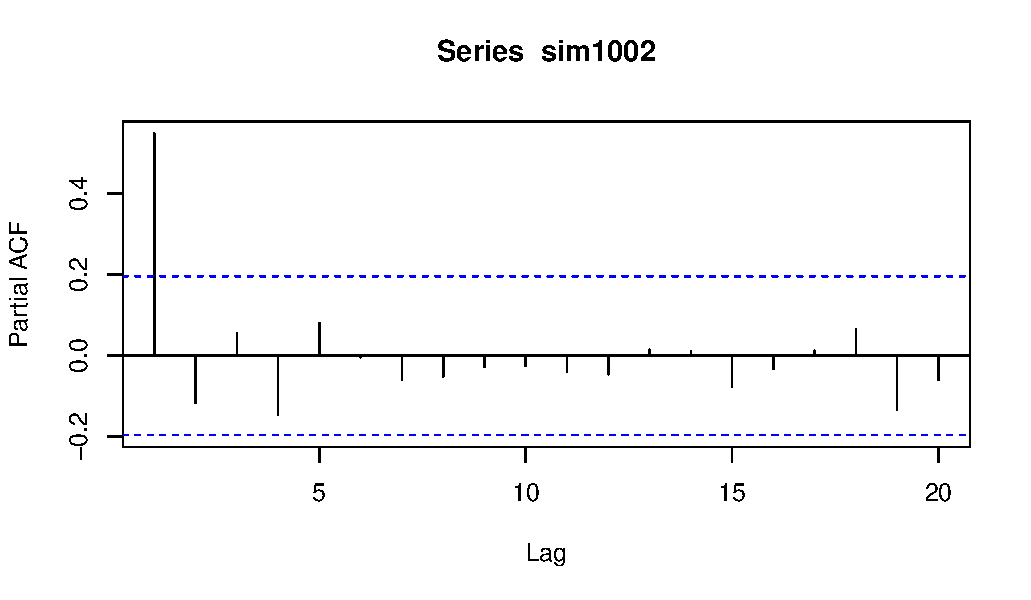
\includegraphics[scale=0.4]{pacf_obs_squ.pdf}
	\end{center}	 
	%\end{itemize}
 \hfill \includegraphics[scale=0.05]{qletlogo} \href{https://github.com/QuantLet/SFE\_class\_2017/tree/master/SFMqmle}{ SFMqmle}
}
%%%%%%%%%%%%%%%%%%%%%%%%%%%%%%%%%%%%%%%%%%%%%
   \section{MLE}
   %%%%%%%%%%%%%%%%%%%%%%%%%%%%%%%%%%%%%%%%%%%%%%%%%%%%%%%%%%%%%%%%%%%%%%%%%%%%%%%%%%%%%%%%%%%%%%%%%%%%%%%%%%%%%%%%%%%%%%%%
\frame[containsverbatim]{
	\frametitle{Maximum Likelihood Estimation (MLE)}
	
	\begin{itemize}
		\item Assume pdf of  \(\varepsilon_{t}|\mathcal{F}_{t-1}\) normal
		\begin{eqnarray*}
			p(\varepsilon_{t}|\mathcal{F}_{t-1})=\frac{1}{\sqrt{2\pi}\sigma_{t}}\exp\left\lbrace - \frac{\varepsilon_{t}^{2}}{2\sigma_{t}^2}\right\rbrace 
		\end{eqnarray*}
		
		\item Conditional log-likelihood function \(\mathit{l}^{b}(\omega,\alpha)\) :
		\begin{eqnarray*}
			\mathit{l}^{b}(\omega,\alpha)=\sum_{t=2}^{n}\log p\left(\varepsilon_{t}|\mathcal{F}_{t-1} \right) 
		\end{eqnarray*}
		where  \(\mathit{l}^b=\log p \left(\varepsilon_{n},...,\varepsilon_{2}|\varepsilon_{1} \right) \)
	\end{itemize}
}

	%%%%%%%%%%%%%%%%%%%%%%%%%%%%%%%%%%%%%%%%%%%%%%%%%%%%%%%%%%%%%%%%%%%%%%%%%%%%%%%%%%%%%%%%%%%%%%%%%%%%%%%%%%%%%%%%%%%%%%%%
\frame[containsverbatim]{
	\frametitle{Maximum Likelihood Estimation (MLE)}
	
	\begin{itemize}
		\item First order conditions  
		\begin{eqnarray*}
			\sum_{t=2}^{n} \dfrac{\partial \mathit{l}_{t}^{b}}{\partial \omega}=0\\ 
			\sum_{t=q+1}^{n} \dfrac{\partial \mathit{l} _{t}^{b}}{\partial \alpha}=0
		\end{eqnarray*}
		
		\item Under the conditions
		\begin{enumerate}
			\item\(\mathsf{E}[Z_{t}|\mathcal{F}_{t-1}]=0\) and \(\mathsf{E}[Z_{t}^{2}|\mathcal{F}_{t-1}]=1\)
			\item\(\mathsf{E}[\log(\alpha Z_{t}^{2})|\mathcal{F}_{t-1}]<0\)(strong stationarity)
		\end{enumerate}
		ML estimators are consistent   
	\end{itemize}
}
%%%%%%%%%%%%%%%%%%%%%%%%%%%%%%
  \section{QMLE}
%%%%%%%%%%%%%%%%%%%%%%%%%%%%%%%%%%%%%%%%%%%%%%%%%%%%%%%%%%%%%%%%%%%%%%%%%%%%%%%%%%%%%%%%%%%%%%%%%%%%%%%%%%%%%%%%%%%%%%%%
\frame[containsverbatim]{
	\frametitle{Quasi Maximum likelihood Estimation (QMLE)}
	\begin{itemize}
		\item Quasi ML (QML): In the case \(Z_{t}\) is not normally distributed, \(\hat{\theta}\) is consistent, and asymptotically normally distrubuted.
	
		\item However, the estimates are not efficient and "the efficiency loss can be marked under asymmetric ... distributions" (Bollerslev and Wooldridge (1992), p. 166). The robust variance-covariance matrix of the estimates equals the (Eicker-White) sandwich estimator, i.e.
		\begin{eqnarray}
		\sqrt{n}(\hat{\theta}-\theta)\xrightarrow{\mathcal{L}}N(0,J^{-1}IJ^{-1})
		\end{eqnarray}
	\end{itemize}
}

%%%%%%%%%%%%%%%%%%%%%%%%%%%%%%%%%%%%%%%%%%
%%%%
\frame[containsverbatim]{
	\frametitle{QQ Plot of standardized residuals}
\begin{center}
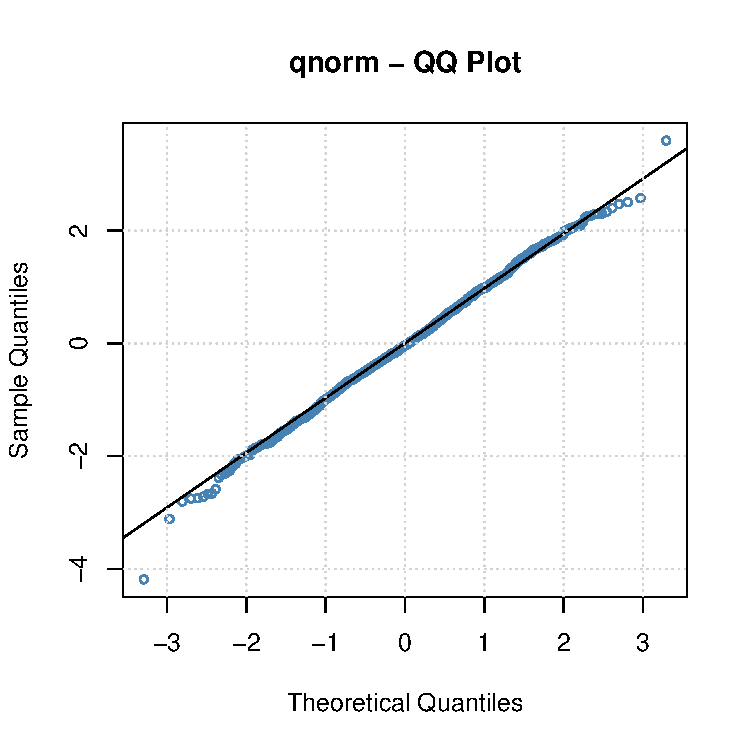
\includegraphics[scale=0.35]{std_res_qqplot.pdf}
\end{center}
	 \hfill \includegraphics[scale=0.05]{qletlogo} \href{https://github.com/QuantLet/SFE\_class\_2017/tree/master/SFMqmle}{ SFMqmle}
}
%%%%%%%%%%%%%%%%%%%%%%%%%%%%%%%%%%%%%%%%%%%%%5
\section{Monte Carlo Simulation}
%%%%%%%%%%%%%%%%%%%%%%%%%%%%%%%%%%%%%%%%%%%%%%%%%%%%%%%%%%%%%%%%%%%%%%%%%%%%%%%%%%%%%%%%%%%%%%%%%%%%%%%%%%%%%%%%%%%%%%%%

% Subsections are not visible on the actual slide, but are displayed as bookmarks in the pdf file. Their application facilitates an easy navigation trough large pdf files.
%%%%%%%%%%%%%%%%%%%%%%%%%%%%%%%%%%%%%%%%%%%%%%%%%%%%%%%%%%%%%%%%%%%%%%%%%%%%%%%%%%%%%%%%%%%%%%%%%%%%%%%%%%%%%%%%%%%%%%%%
\subsection{Motivation}
%%%%%%%%%%%%%%%%%%%%%%%%%%%%%%%%%%%%%%%%%%%%%%%%%%%%%%%%%%%%%%%%%%%%%%%%%%%%%%%%%%%%%%%%%%%%%%%%%%%%%%%%%%%%%%%%%%%%%%%%

%%%%%%%%%%%%%%%%%%%%%%%%%%%%%%%%%%%%%%%%%%%%%%%%%%%%%%%%%%%%%%%%%%%%%%%%%%%%%%%%%%%%%%%%%%%%%%%%%%%%%%%%%%%%%%%%%%%%%%%%
\frame{
	\frametitle{Requirements}
	
	\begin{itemize}
		\item Control over the random variables and parameters (selection of pdf for random numbers)
		\item Reproducibility
		\item Efficiency
		\item Documented steps
		
	\end{itemize}
}
\section{Monte Carlo Set up}
%%%%%%%%%%%%%%%%%%%%%%%%%%%%%%%%%%%%%%%%%%%%%%%%%%%%%%%%%%%%%%%%%%%%%%%%%%%%%%%%%%%%%%%%%%%%%%%%%%%%%%%%%%%%%%%%%%%%%%%%

% Subsections are not visible on the actual slide, but are displayed as bookmarks in the pdf file. Their application facilitates an easy navigation trough large pdf files.
%%%%%%%%%%%%%%%%%%%%%%%%%%%%%%%%%%%%%%%%%%%%%%%%%%%%%%%%%%%%%%%%%%%%%%%%%%%%%%%%%%%%%%%%%%%%%%%%%%%%%%%%%%%%%%%%%%%%%%%%
\subsection{Monte Carlo Set up}
%%%%%%%%%%%%%%%%%%%%%%%%%%%%%%%%%%%%%%%%%%%%%%%%%%%%%%%%%%%%%%%%%%%%%%%%%%%%%%%%%%%%%%%%%%%%%%%%%%%%%%%%%%%%%%%%%%%%%%%%

%%%%%%%%%%%%%%%%%%%%%%%%%%%%%%%%%%%%%%%%%%%%%%%%%%%%%%%%%%%%%%%%%%%%%%%%%%%%%%%%%%%%%%%%%%%%%%%%%%%%%%%%%%%%%%%%%%%%%%%%
\frame{
	\frametitle{Monte Carlo Set up}
	
	\begin{itemize}
	\item R-Package: fGarch\\
	\item Testing for different RNG: Mersenne Twister,Knuth-TAOCP-2002, Wichmann-Hill with seed=123.\\
	\item Custom function called 'simulation' which takes as input size of the dataset and returns the string of:
	\begin{enumerate}
		\item averaged value of estimated $\hat{\alpha}$ 
		\item standard deviation of estimated $\hat{\alpha}$ from true parameter $\alpha$ = 0.9
		\item number of $\hat{\alpha}$ which are larger or equal to 1 (evidence of the stationarity violation)
	\end{enumerate}
	\end{itemize}
	over \(\mathit{k}=1000\) replications for datasets of size \(\mathit{n}=100,250,500,1000\).
}
\frame{
	\frametitle{Monte Carlo Set up continued}
	Functions used: 
\begin{itemize}
	\item fitGarch() with specified conditional distribution to be calculated with the Quasi Maximum Likelihood Estimation;
	 \item garchSim() for simulation of ARCH(1) models.
\end{itemize} 
}

%%%%%%%%%%%%%%%%%%%%%%%%%%%%%%%%%%%%%%%%%%%%%%%%%%%%%%%%%%%%%%%%%%%%%%%%%%%%%%%%%%%%%%%%%%%%%%%%%%%%%%%%%%%%%%%%%%%%%%%%

\section{Simulation Results}
%%%%%%%%%%%%%%%%%%%%%%%%%%%%%%%%%%%%%%%%%%%%%%%%%%%%%%%%%%%%%%%%%%%%%%%%%%%%%%%%%%%%%%%%%%%%%%%%%%%%%%%%%%%%%%%%%%%%%%%%
\frame{
	\frametitle{Results of Monte Carlo Simulation}
	\vspace{-0.5cm}
	\begin{table}
	\begin{center}
		\begin{tabular}{cccr}
			\hline\hline
			\textit{n}& $k^-1\sum_{j=1}^k \hat{\alpha_j}$ & $\sqrt{k^-1\sum_{j=1}^k (\hat{\alpha_j}-\alpha)^2}$ & $ \# (\alpha_j \geq 1) $ \\
			\hline
			100 & 0.824 & 0.209 & 34.5\%  \\
			250           & 0.868 & 0.130 & 23.2\%  \\
			500           &0.880 & 0.095 & 17.3\%  \\
		   1000     &0.890 & 0.073 & 7.4\%  \\
		\hline\hline
	\end{tabular}
    \caption{RNG: Mersenne Twister}
	\end{center}
    \end{table}

   \hfill \includegraphics[scale=0.05]{qletlogo} \href{https://github.com/QuantLet/SFE\_class\_2017/tree/master/SFMqmle}{ SFMqmle}
	%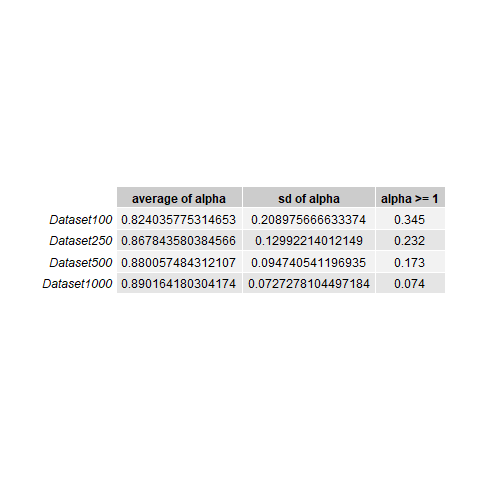
\includegraphics[scale=0.2]{C:/Users/paulina/Desktop/TeXBeamer/table 2017_12_16 205928 set seed 123 Marsenne Twister.png}

}


\frame{
	\frametitle{Results with other RNG}
		\vspace{-0.5cm}
   \begin{table}
	\begin{center}
		\begin{tabular}{cccr}
			\hline\hline

			\textit{n}            & $k^-1\sum_{j=1}^k \hat{\alpha_j}$ & $\sqrt{k^-1\sum_{j=1}^k (\hat{\alpha_j}-\alpha)^2}$ & $ \# (\alpha_j \geq 1) $ \\
			\hline
			100 & 0.820 & 0.207 & 30.1\%  \\
			250           & 0.869 & 0.128 &24.1\%  \\
			500           &0.883 & 0.097 & 17.2\%  \\
			1000     &0.890 & 0.072 & 9.3\%  \\
		\hline\hline
	\end{tabular}
    \caption{RNG: Knuth-TAOCP-2002}
	\end{center}
\end{table}
\hfill \includegraphics[scale=0.05]{qletlogo} \href{https://github.com/QuantLet/SFE\_class\_2017/tree/master/SFMqmle}{ SFMqmle}
}

\frame{
	\frametitle{Results with other RNG}
	
    \begin{table}
	\begin{center}
		\begin{tabular}{cccr}
			\hline\hline
			\textit{n}            & $k^-1\sum_{j=1}^k \hat{\alpha_j}$ & $\sqrt{k^-1\sum_{j=1}^k (\hat{\alpha_j}-\alpha)^2}$ & $ \# (\alpha_j \geq 1) $ \\
			\hline
			100 & 0.822 & 0.207 & 31.1\%  \\
			250           & 0.868 & 0.132 &24.5\%  \\
			500           &0.884 & 0.096 & 17.9\%  \\
			1000     &0.896 & 0.070 & 9.7\%  \\
			\hline\hline
		\end{tabular}
	\caption{RNG: Wichmann-Hill}
	\end{center}
    \end{table}
\hfill \includegraphics[scale=0.05]{qletlogo} \href{https://github.com/QuantLet/SFE\_class\_2017/tree/master/SFMqmle}{ SFMqmle}
}
%%%%%%%%%%%%%%%%%%%%%%%%%%%%%%%%%%%%%%%%%%%%%%%%%
%%%%%%%%%%%%%%%%%%%%%%%%%%%%%%%%%%%%%%%%%%%%%%%%%%%%%
\section{Further Information}

\frame{
	\frametitle{For Further Reading}
   	\begin{thebibliography}{aaaaaaaaaaaaaaaaa}
		\beamertemplatearticlebibitems
	    \bibitem{gentle4elements}
	    James~E Gentle.
	    \newblock Elements of computational statistics.
	    \newblock {\em QA276}, 4:G455.
		\beamertemplateonlinebibitems
		\bibitem{wuertz2008fgarch}
		D~Wuertz, Y~Chalabi, and M~Miklovic.
		\newblock fgarch: Rmetrics-autoregressive conditional heteroskedastic
		modelling, r package version 290.76, 2008
		\beamertemplatebookbibitems
		\bibitem{franke2004statistics}
		J{\"u}rgen Franke, Wolfgang~Karl H{\"a}rdle, and Christian~M Hafner.
		\newblock {\em Statistics of financial markets}
		\newblock Forth Edition, Springer-Verlag Berlin Heidelberg, 2015.
	\end{thebibliography}
}
\end{document}
